
\section{Synchronization Topologies}
\label{sec:histo.topologies}

In this section we will look at different network topologies to evaluate how they are supported by our synchronization protocol.
We will further explore options for optimization of our protocol with regards to each topology.
The focus will be on optimizing difference computation and minimizing the length of commit history that has to be stored on collaborating nodes.

\subsection{Master - Client}
\label{sec:histo.topologies.master-client}
In a Master-Client or Client-Server setup we have a single server that handles all data propagation.
The clients can only synchronize their data with the server and directly with each other.
With regards to our synchronization protocol, this means each client has to remember only one remote tracking head.\\
We can optimize our protocol by adding a data pruning step.
As explained in section \ref{sec:histo.protocol}, each commit corresponds to a synchronization point between two nodes.
As we only synchronize with the server, the ancestor commit of a client's head is always equal to the client's remote tracking head of the server.
We can therefore prune all data on the client that is neither part of our branch head nor the remote tracking head.
Pruning is defined as deleting all objects in our store whose hashes are not referenced in the data hierarchy of the commits we want to keep.
We effectively only keep our current data and the data we received last from the server.
In terms of memory usage of the client's store, this topology is therefore the most efficient one.\\
The same is true for the computation of commit and data differences as described in Section \ref{sec:histo.diff-across-commits}.
Running the protocol with the client as the source and the server as the target, the lowest common ancestor of the source's head and the source's remote tracking head is always the remote tracking head itself.
We therefore only need to compute the commit difference between the current head and the ancestor commit, which is the remote tracking head.\\
These optimizations do not apply for running the protocol with the server as the source and the client as the target.
The server could have synchronized with other client nodes in the meantime, which means that its head is more than one commit ahead of the client.\\
We can still apply a data pruning optimization to the server by letting the server forget the commit history that goes beyond the least recently synchronized client.
The more frequently the clients synchronize the more space efficient the protocol becomes.\\
Figure \ref{fig:histo.topologies.client-server} illustrates a possible state in a client-server setup.

\begin{figure}[H]
  \centering
  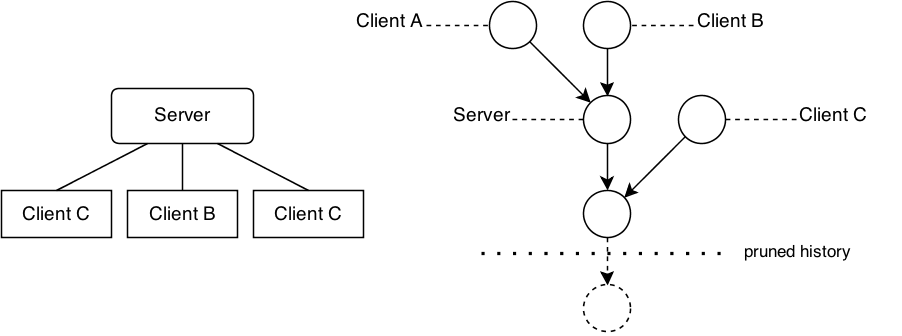
\includegraphics[width=0.9\textwidth]{img/client-server}
  \caption{Client-Server topology with history data pruned at least recently synchronized node.}
  \label{fig:histo.topologies.client-server}
\end{figure}

\subsection{Client - Client}
\label{sec:histo.topologies.p2p}
A client-client or peer-to-peer topology is the opposite extreme of a client-server setup.
Every client can directly synchronize with any other client.
On a network with $ n $ nodes, each node potentially synchronizes with $ n - 1 $ other nodes and therefore has to remember $ n - 1 $ remote tracking heads.\\
We can still apply some optimizations in the form of data pruning.
Let $ A $ be the remote tracking head with the largest distance to a node's head.
All data that is not part of any commit between a node's own head and the lowest common ancestor with $ A $ can be deleted.
It means we only keep the data history until the state of the most outdated node in the network.\\
To maximize the efficiency of this pruning technique, we have to ensure that each node on the system has the best possible information on other node's heads.
We can therefore extend our synchronization protocol to not only set the source's head as the remote tracking head on the target node but to also update all other remote tracking head's using the source's information.
For each remote tracking head $ A $ of the source node, we compute the lowest common ancestor $ C $ of the corresponding tracking head $ B $ on the target node.
If $ C $ is equal to $ A $, we know that our information on the node's head is more up to date.
If $ C $ is equal to $ B $, the source node has more current information and we update the target's remote tracking head to $ A $.
This ensures that the information on remote node heads will eventually propagate across all collaborating nodes.\\

\begin{figure}[H]
  \centering
  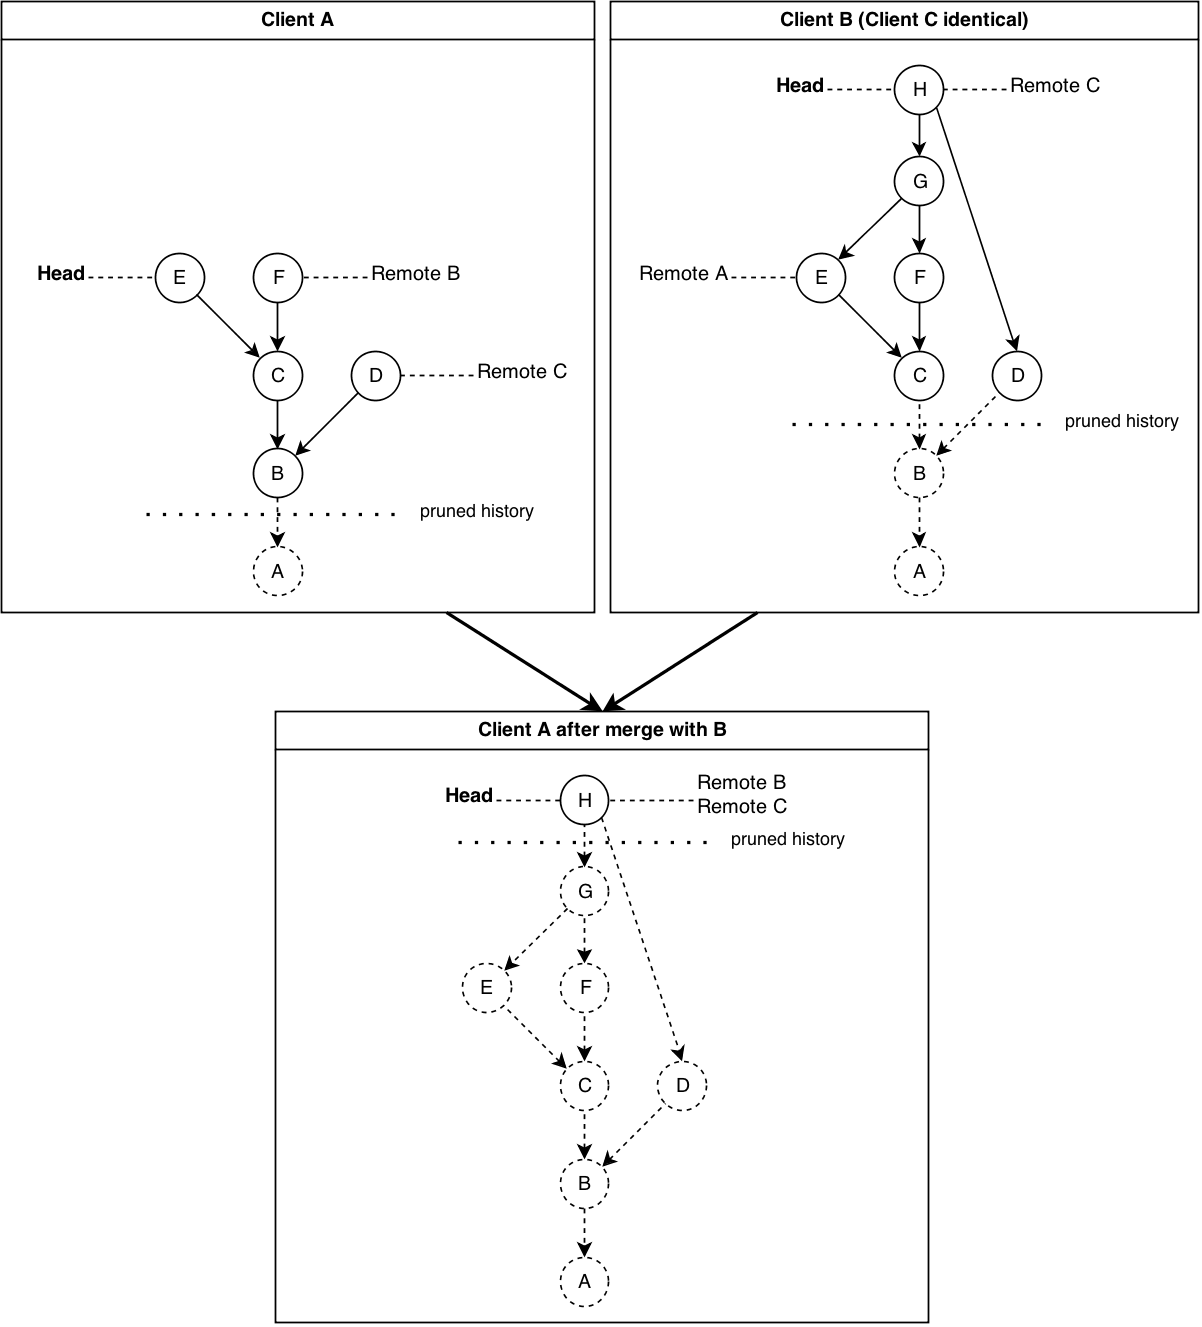
\includegraphics[width=1.0\textwidth]{img/client-client}
  \caption{Client-Client topology showing a merge of three clients.}
  \label{fig:histo.topologies.client-client}
\end{figure}

In Figure \ref{fig:histo.topologies.client-client} we have an examplaric merge of three clients.
\emph{Client A's} head is intially at $ E $ as it has not recently synchronized data from \emph{client B} or \emph{client C}.
\emph{Client B} has already synchronized changes from both \emph{client A} and \emph{client C}.
\emph{Client C} has synchronized changes from \emph{client B} and therefore does not have to pull changes from \emph{client A} anymore.
Note that as the synchronization has to be repeated for both directions, the fact that \emph{client B} has synchronized data from \emph{client A} does not imply that the reverse is true.
Due to network partitions it is possible that \emph{client A} did not hav enough time to synchronize changes from \emph{client B}.\\
We can see that the respective clients track the head of remote nodes.
\emph{Client A's} knowledge about the heads of \emph{client B} and \emph{client C} is obviously outdated.
The client therefore only prunes history after \emph{commit B} as he would otherwise lose the common ancestor with \emph{client C}.\\
\emph{Client B} and \emph{client C} already know that their common ancestor with \emph{client A} is at \emph{commit C} and can therefore prune \emph{commit B}.\\
In a next step \emph{client A} synchronizes data from \emph{client B} and can fast-forward his head to \emph{commit H}.
He also learns that \emph{client C's} head is already at \emph{commit H} and can therefore prune the entire history after \emph{commit H}.

\subsection{Multi Master - Client}
\label{sec:histo.topologies.multi-master}
In a multi master-client setup we have a set of servers that synchronize with each other and a set of clients who can synchronize with any server.
The servers synchronize in a peer-to-peer topology with each other, while the clients cannot communicate with each other.\\
The advantage of this setup over a pure client-server setting is that we can distribute the synchronization load across multiple servers.
Each server is only responsible for a subset of clients.
The data is kept-up-to date across all servers by synchronizing them with each other in regular intervals.\\
The server's can only make use of the peer-to-peer optimizations described in the previous section.
The client's can make full use of the client-server optimizations we described in Section \ref{sec:histo.topologies.master-client} as long as they always connect to the same server.\\
If a client first synchronizes with server $ A $ and then $ A $ gets replaced with server $ B $, we have a race condition if the client does not realize the server has changed.
$ B $ might not have the latest changes the client sent to $ A $ if $ A $ and $ B $ have not synchronized in the meantime.
The client still thinks that its remote tracking head of the server is correct.\\
This is a very unlikely event as the servers are usually connected with much lower latency than the client with the server.
Our synchronization protocol is robust enough so that synchronization will still succeed.
Propagation from the server to the client will only be less efficient.
The commit difference of the server will contain all commits in its history if the client's remote tracking head is not actually stored on the server.
While this means that some redundant metadata is sent between the nodes, the computation of the actual data difference is still efficient.
Sections \ref{sec:histo.protocol.detection-propagation} and \ref{sec:histo.diff-across-commits} describe the data propagation protocol in detail.

\subsection{Hierarchical}
In a hierarchical topology we consider the situation of clients being connected to different networks.
Figure \ref{fig:histo.topologies.hierarchical} shows an example for a simple hierarchical setup.
Being in an office environment, the clients are all connected to a local network usually via Wi-Fi.
The local network in turn connects the clients to the internet but also allows them to directly connect to other nodes on the local network.
We could therefore run an `office server' in the local network, allowing the clients to synchronize with low-latency in a client-server topology.\\

\begin{figure}[H]
  \centering
  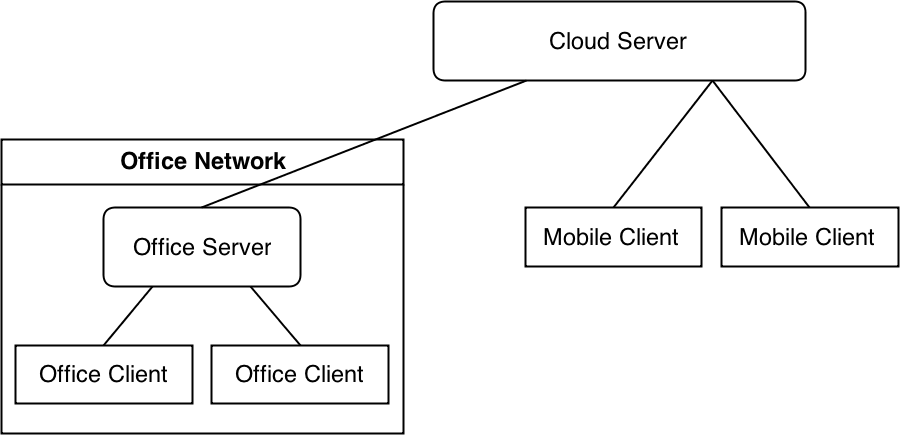
\includegraphics[width=0.8\textwidth]{img/hierarchical}
  \caption{Hierarchial synchronization topology.}
  \label{fig:histo.topologies.hierarchical}
\end{figure}

Users working from home or travelling still want to be able to synchronize with their colleagues.
We add a `cloud server' to our topology, which runs in an internet server farm.
The cloud server continuously synchronizes with the office server as described for the multi-master setup.
Mobile nodes can now synchronize with the cloud server allowing them to propagate updates from and to the nodes in the office network.\\
Due to the continuous connection between the office and the cloud server we can let the clients see both servers as the same and apply the same optimizations as for the client-server setup.
As in the previous topology there is a race condition when synchronizing with the different servers, which can in rare cases result in a slightly inefficient data propagation.\\
If we choose to let the clients track both servers as different remotes, we can only apply the optimization described for the peer-to-peer setup in Section \ref{sec:histo.topologies.p2p}.
This is still a very efficient solution as the two server nodes are unlikely to differ much in their branch heads.
